%开普勒三定律

\pentry{椭圆的三中定义\upref{Elips3}}

开普勒定律描述了行星围绕固定中心天体的运动的规律. 第一定律给出了行星运动轨道的几何形状, 第二定律描述了行星在轨道不同位置的相对速度, 第三定律给出周期与轨道长轴的关系. 开普勒三定律最早是开普勒根据对太阳系中行星的观测数据总结而来的, 但牛顿运用他的第二定律\upref{New3} 和万有引力定律\upref{Gravty}, 将开普勒三定律精确地推导了出来.

\bb{第一定律}: 每一个行星都沿各自的椭圆轨道环绕中心天体, 中心天体则处在椭圆的一个焦点上.
\begin{figure}[ht]
\centering

\includegraphics[width=3.7cm]{./figures/Keple1.pdf}
\caption{开普勒第一定律} \label{Keple_fig1}
\end{figure}

\bb{第二定律}:相等时间内, 中心天体与行星的连线所扫过的面积是相等的.
\begin{figure}[ht]
\centering
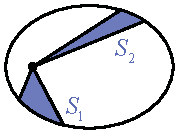
\includegraphics[width=3.3cm]{./figures/Keple2.pdf}
\caption{开普勒第二定律} \label{Keple_fig2}
\end{figure}

\bb{第三定律}: 椭圆轨道半长轴($a$)的立方与周期(公转一圈所用的时间 $T$)的平方成正比.

\subsection{数值模拟及证明}

以下的推导中, 需要忽略行星与恒星的大小, 行星之间的相互引力以及中心天体的运动. 在进行解析推导之前, 不妨先看看更为直观的数值模拟.
 
\begin{itemize}
\item 天体运动的简单数值计算\upref{KPNum0}
\item 开普勒第一定律的证明\upref{Keple1}
\item 开普勒第二定律的证明\upref{Keple2}
\item 开普勒第三定律的证明\upref{Keple3}
\end{itemize}
 
%说明行星运动的周期只跟中心天体质量有关.特别要强调的是,如果考虑中心天体的运动, 开普勒一,二定律仍然成立, 但第三定律却不一定成立, 具体原因见下文"考虑中心天体运动所做的修正".
